\section{Background}
Nick Week 1

Recently, a new exciting \remove{and much needed} segment of the technology sector \change{as}{has} sprung up – indoor navigation with a catalyst of growth in indoor navigational research. Most current solutions on the market cater very well for a basic navigation of large open public spaces, \change{fail}{but failing} to display a competency of more complex navigational requirements coupled with an even proportion of navigational and interactive content with well-presented data. Through the use of augmented reality, the concept can provide an interactive \remove{navigation} solution for museums and exhibitions – with a wide future scope. \note{I like this a lot!}

Since most museums and galleries use a portable audio guide, user experiences can be vastly improved by the use of a phone. Currently only a few solutions can be found; the Orpheo group \cite{orpheo} provide a unique app for each place meaning that their solution is somewhat cumbersome to regular museum users who would wish to have a hassle-free setup process. As we hope to appeal to museums and by virtue of this, museum-goers, having one app whereby the user can simply walk into a museum or exhibition and be greeted with relevant information to be a vital differentiating factor \cite{microsoft}. Even though the intention is to create one app for every museum and exhibition for the project, each client would have a large input on the content of their institution within the app. 

If a museum, wanted a solution for navigation, due to the low number of museum-specific competitors, would choose to use a standard indoor map- ping software \cite{murphy}. However, while there are many options out there from Google and Mapspeople \cite{mapspeople} who set out to provide this, they lack important exigences that are very imperative for museums like heavily integrated augmented reality, intelligent tour guiding from your location, and virtual reality to take a scene from the museum, for instance, and place the user to the artefact’s original time and place. 
\note{could you summarise and add in one paragraph the studies that Hamza researched?}

\section{AR Libraries}
Gabe Week 1

\note{Not a huge fan of these lists, not very academic in style, and too bullet pointy. also say in one line for each, what they do}
As exemplified in the following list, \note{don't write in first person} we had a large variety of libraries to choose from: 
\begin{itemize}
    \item Apple ARKit (iOS)
    \item AR Core (Android)
    \item Vuforia (Unity/Android)
    \item Wikitude (Android)
    \item EasyAR (iOS \& Android)
    \item ARToolKit (Unity)
\end{itemize}
However, after the brief evaluation of each. Our focus was shifted onto  Apple's ARKit, Android's ARCore and Vuforia because ARCore and ARKit are native to \change{our}{their} prospective platforms. Making them ideal choices for development, regardless of which platform we would end up on. Vuforia has unrivalled documentation so as a cross-platform choice, it outshines the others for the task that needed to be completed. \note{talk about how popular unity is}

% \subsection{Development Platforms}
To optimise our development process, it was clear that \note{don't write in first person} we needed to focus our efforts on developing for one platform from the following three choices: Android, iOS and Unity. Each of which had advantages and disadvantages that would distinguish which one we would choose.

\note{remove the lists and use paragraphs}
\begin{itemize}
    \item iOS: Is a popular platform, making it a choice worthy of thorough analysis. Unlike android has more comprehensive documentation and \change{an easy}{a shallow} learning-curve. But due to it being an \annote{isolated platform}{doesn't make sense}, \annote{it would be difficult to develop on since it would be difficult to refer to outside documentation}{doesn't make sense}. 
    \item Unity: Is the more niche, but simple development platform of the three. It has unique resources that the other two cannot have because of its cross-platform nature \note{such as...}, however its unfamiliarity to the group and stakeholders, and steep learning curve made it unfit as a platform for development.
    \item Android: Would allow the entire group to develop more flexibly \note{talk more technically}. We have more Android resources available and they were easier to get a hold of. \change{Its}{It is} also the most familiar platform to the development team, and to the stakeholders. Making it the reason why we chose this as the main development platform.
\end{itemize}

\section{Software Architecture}
Hardik Week 1

\note{Please check the essay plan, you've basically written Gabriel's section!}
In order to identify platforms that are good for implementing AR on smart- phones, prototyping was divided into three platforms to explore them such as Vuforia (Unity/Android), ARKit(iOS) and AR Core (Android). Building test applications to discover how they assist with implementation in our application and what problem will be faced during the implement.

\subsection*{Vuforia (Unity/Android)}
Unity is a cross-platform game engine, used to test a simple AR camera prototype where the device’s camera hovers an image, and displays information about that image on the device. The application was built using Vuforia, an SDK that enables recognition, and tracking of image targets. This library can be used for the exploration case in the use case model. Although, there is a lack of tools for locating user current location compared to Android.

Figure here

% \subsubsection{Vuforia}
% \begin{figure}[H]
% \centering  
% \begin{tabular}{cc}
%   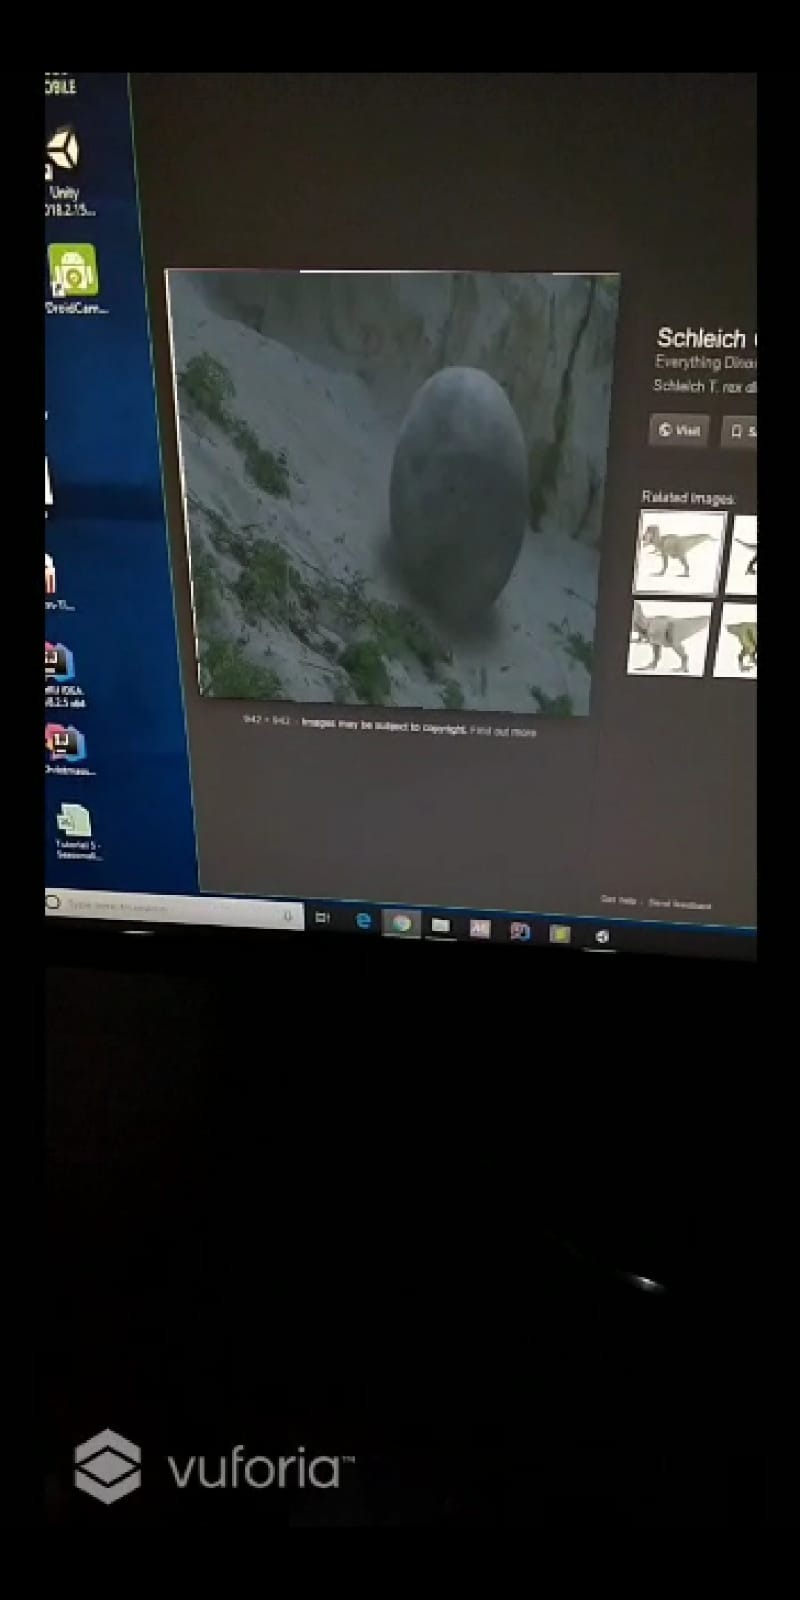
\includegraphics[width=60mm, height=100mm]{prototypes/ar/vulforia/1.jpeg} &   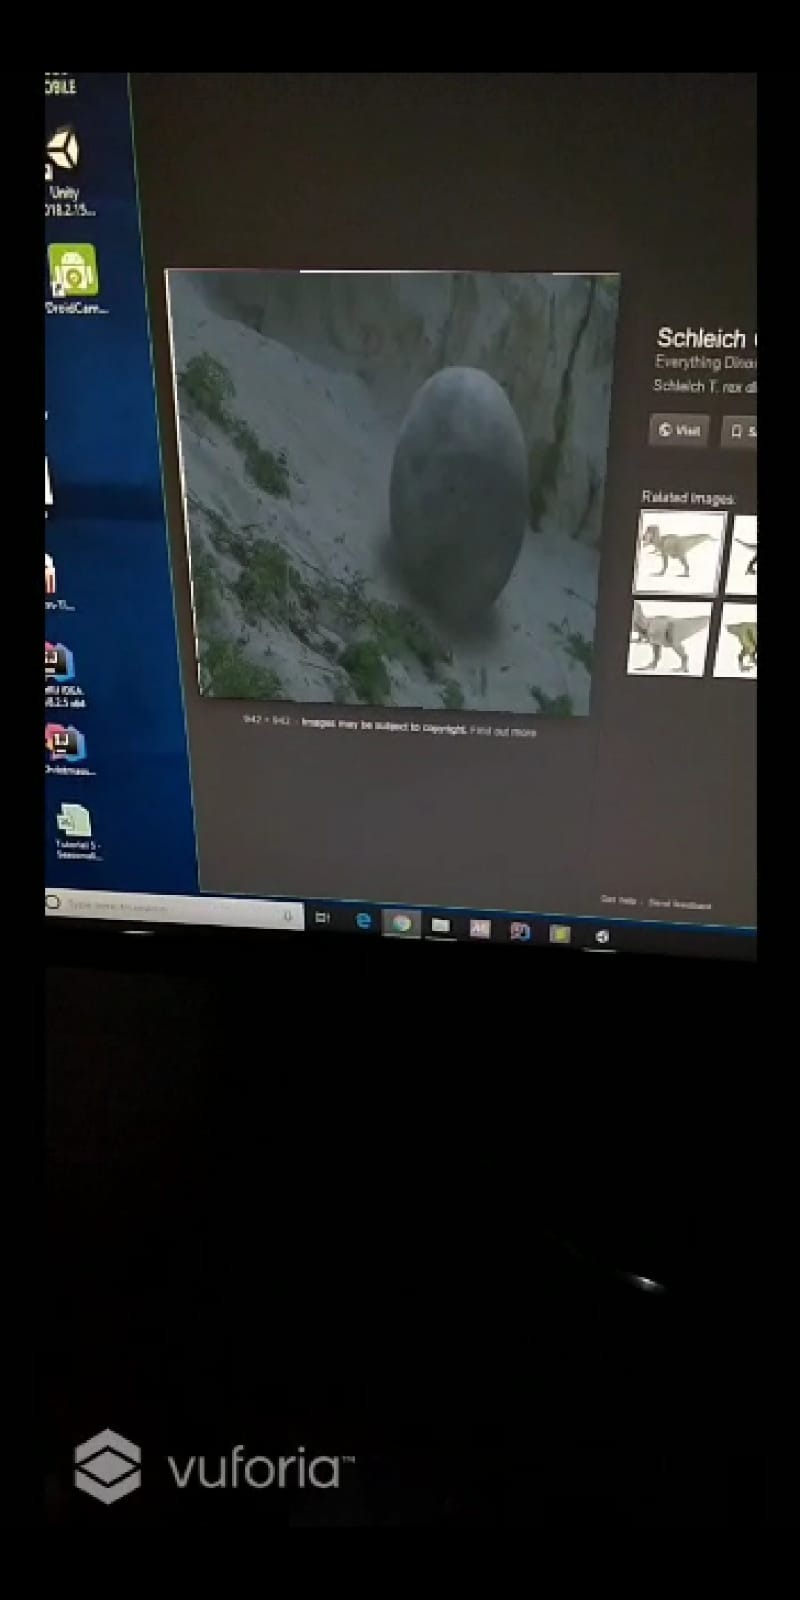
\includegraphics[width=60mm, height=100mm]{prototypes/ar/vulforia/2.jpeg} \\
% (a) Camera over image & (b) Video superimposed on top of image\\[6pt]
% \end{tabular}
% \caption{Vuforia prototyping on Android device}
% \label{fig:vulforia}
% \end{figure}

\subsection*{ARKit (iOS)}
A similar prototype to Unity was built on Apple’s ARKit using Swift [8], which was easy to learn. It was intuitive to implement AR features as there was detailed documentation, but logging GPS data was harder compared to Android therefore we would not able to work with ARKit.

Figure here

% \subsubsection{ARKit}
% \begin{figure}[H]
% \centering  
% \begin{tabular}{cc}
%   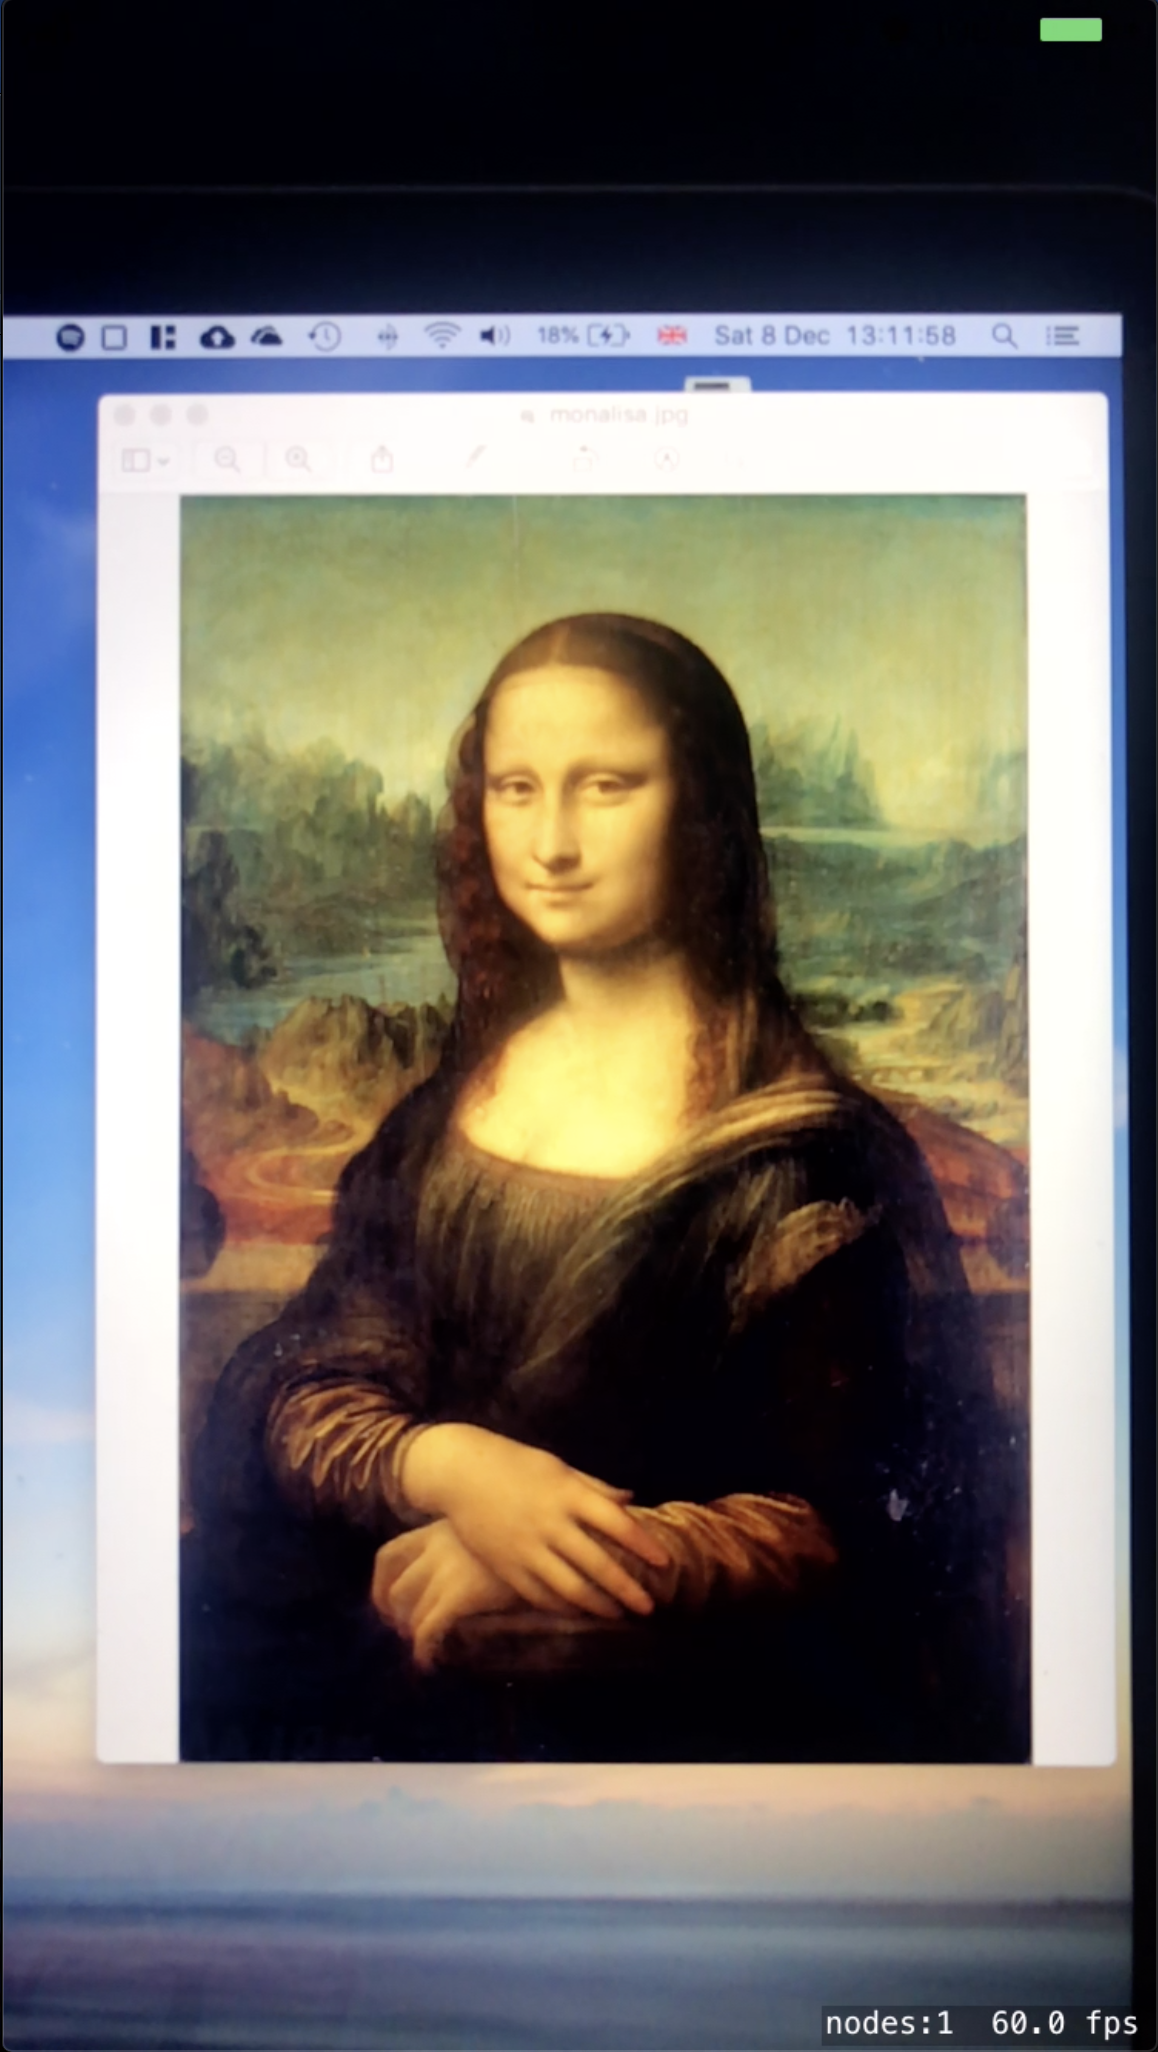
\includegraphics[width=60mm, height=100mm]{prototypes/ar/ios/1.png} &   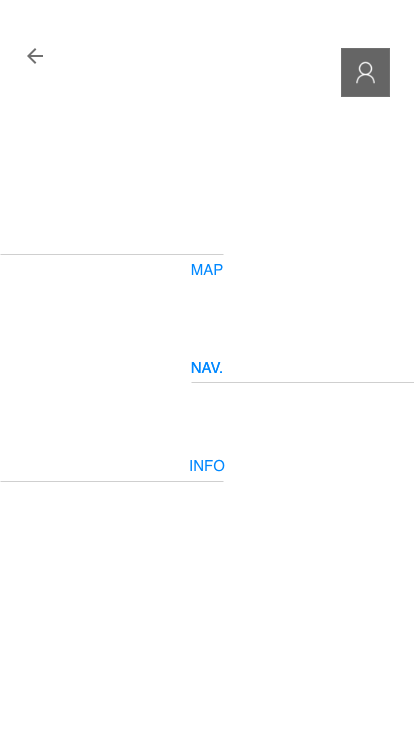
\includegraphics[width=60mm, height=100mm]{prototypes/ar/ios/2.png} \\
% (a) Camera over image & (b) Image recognised and displaying information \\[6pt]
% \multicolumn{2}{c}{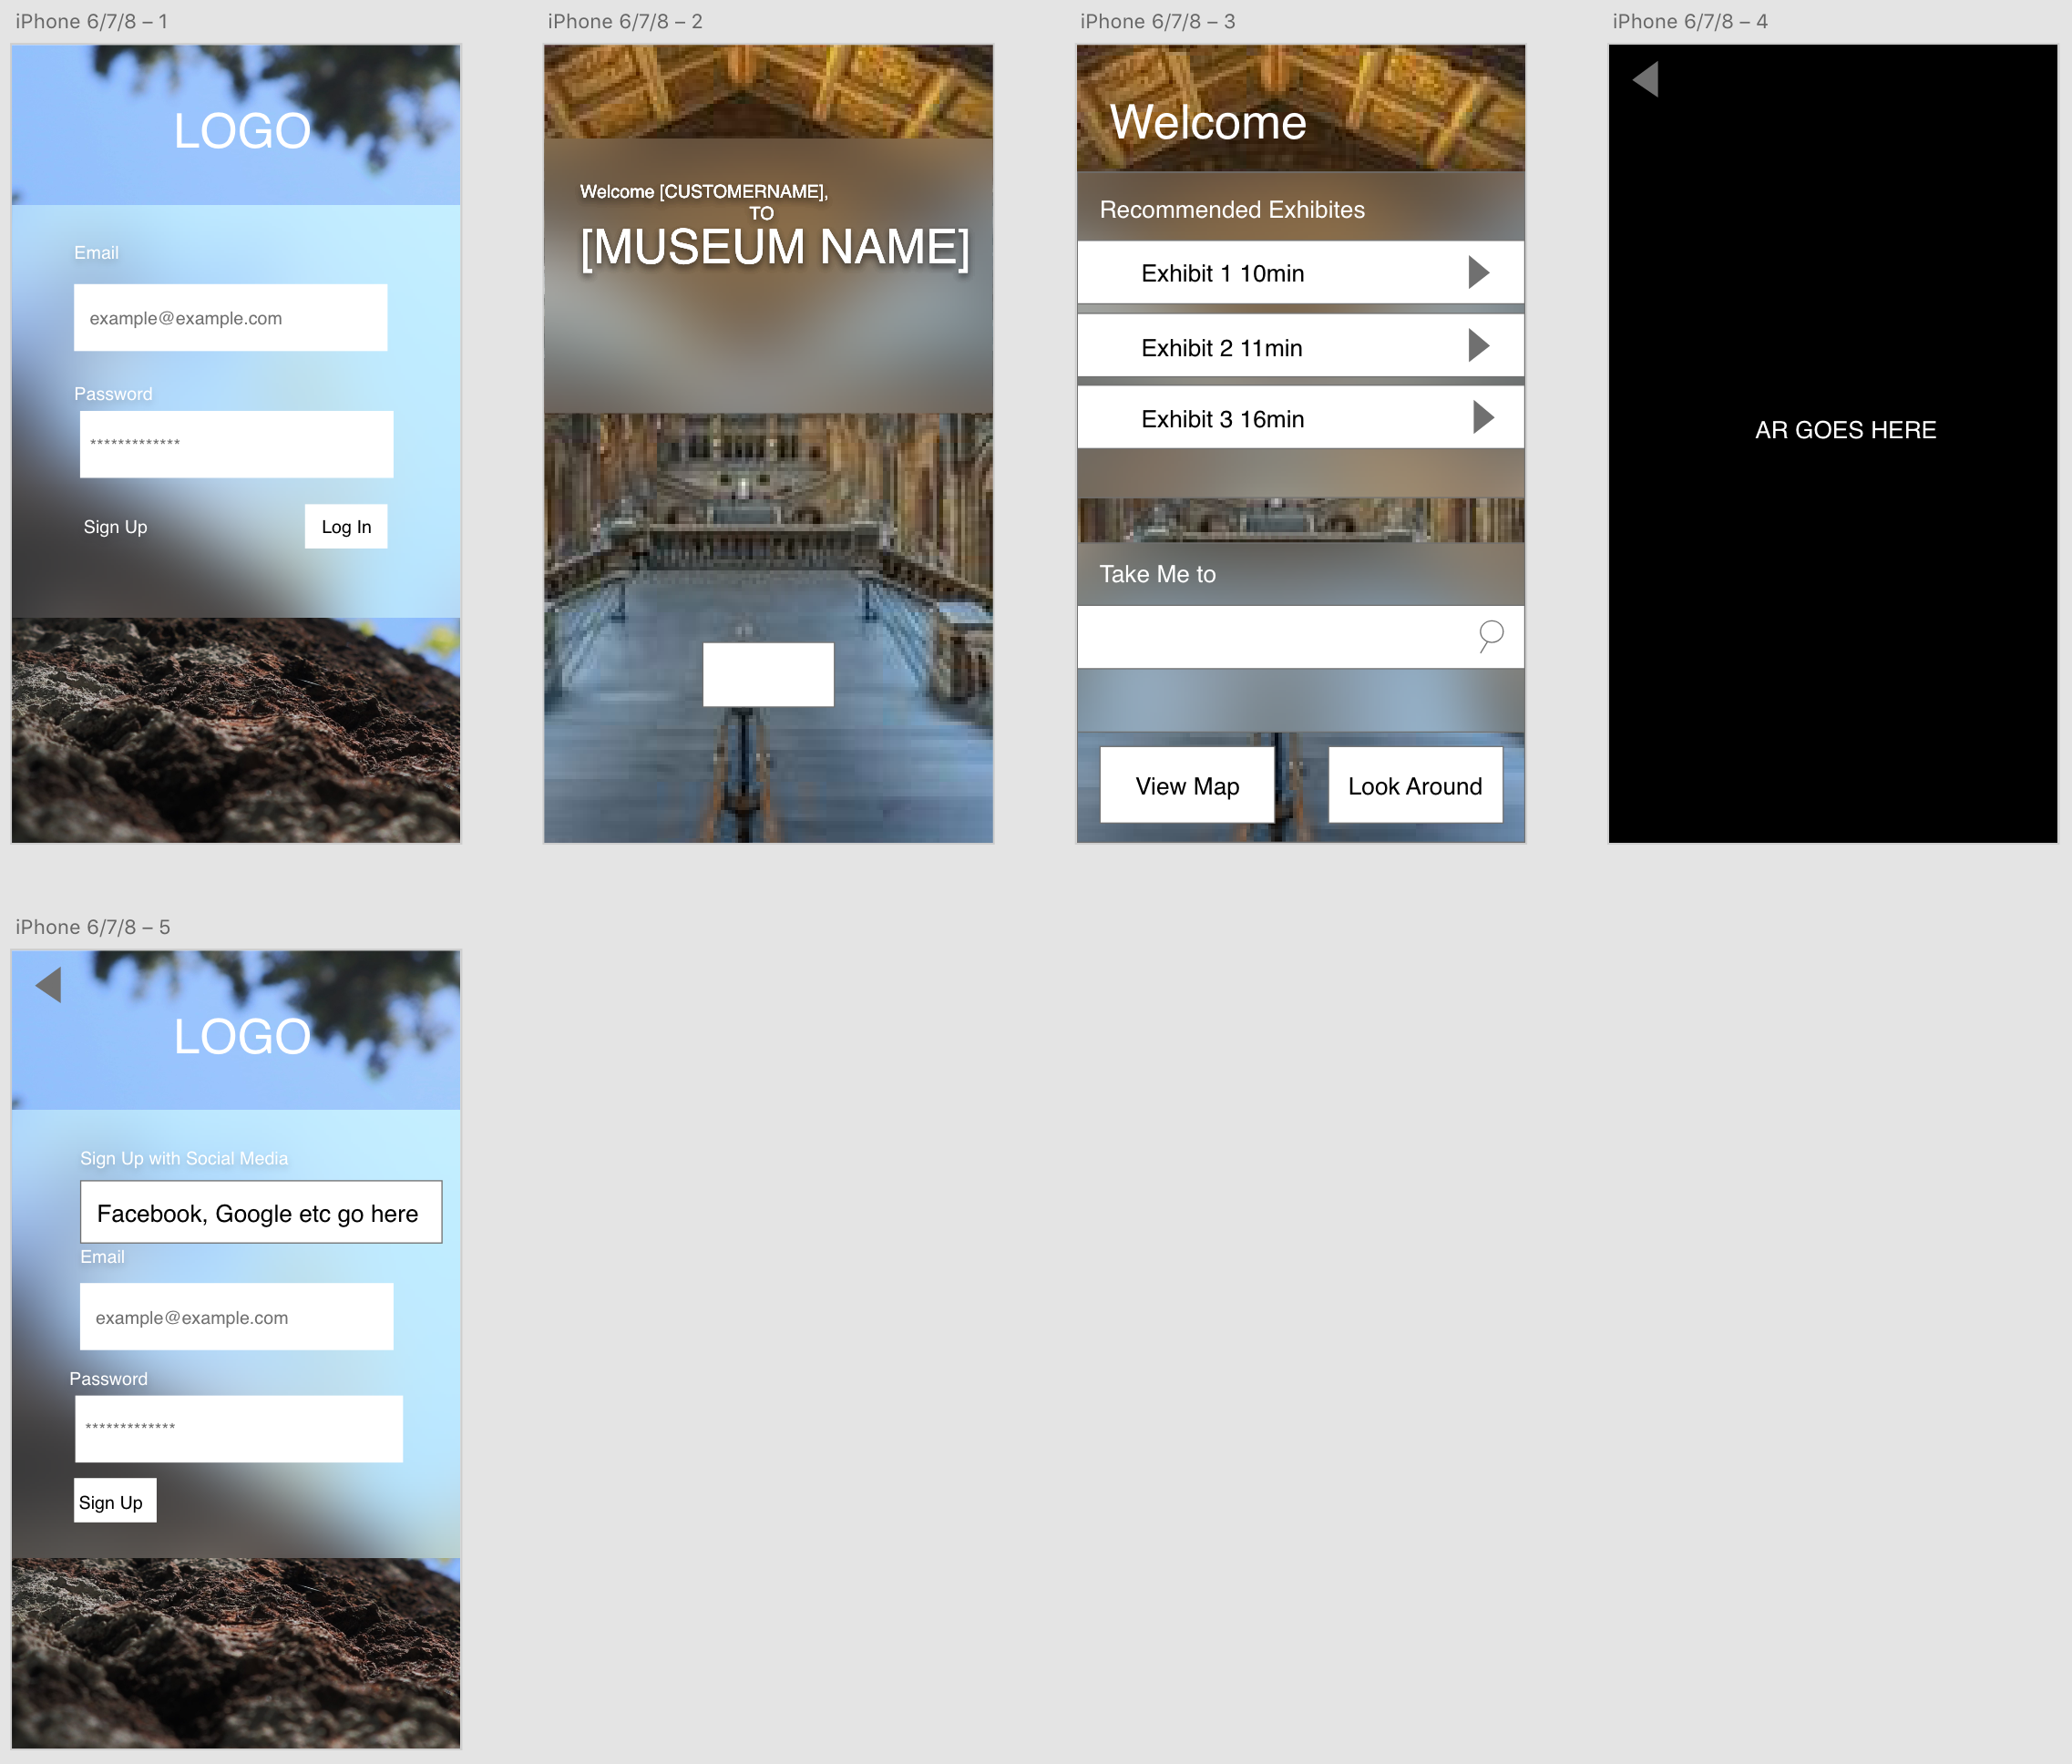
\includegraphics[width=60mm, height=100mm]{prototypes/ar/ios/3.png} }\\
% \multicolumn{2}{c}{(c) Image scanned before; showing the green tick}
% \end{tabular}
% \caption{ARKit prototyping on iOS device}
% \label{fig:ARKit}
% \end{figure}

\subsection*{AR Core (Android)}
ARCore was used to create a simple 3D model showing on a mobile device when its camera targeted flat surface. Compared to iOS, it is easier to log GPS location, although connecting the user interface to the scripts was more challenging.

After exploring this three prototype, we found ARCore(Android) will work best in our AR application. ARCore helps us to identify the user current GPS location therefore our Developer team need to put lot of effort into delivering a right location on user’s screen.

Figure here

% \subsubsection{ARCore}
% \begin{figure}[H]
% \centering  
% \begin{tabular}{cc}
%   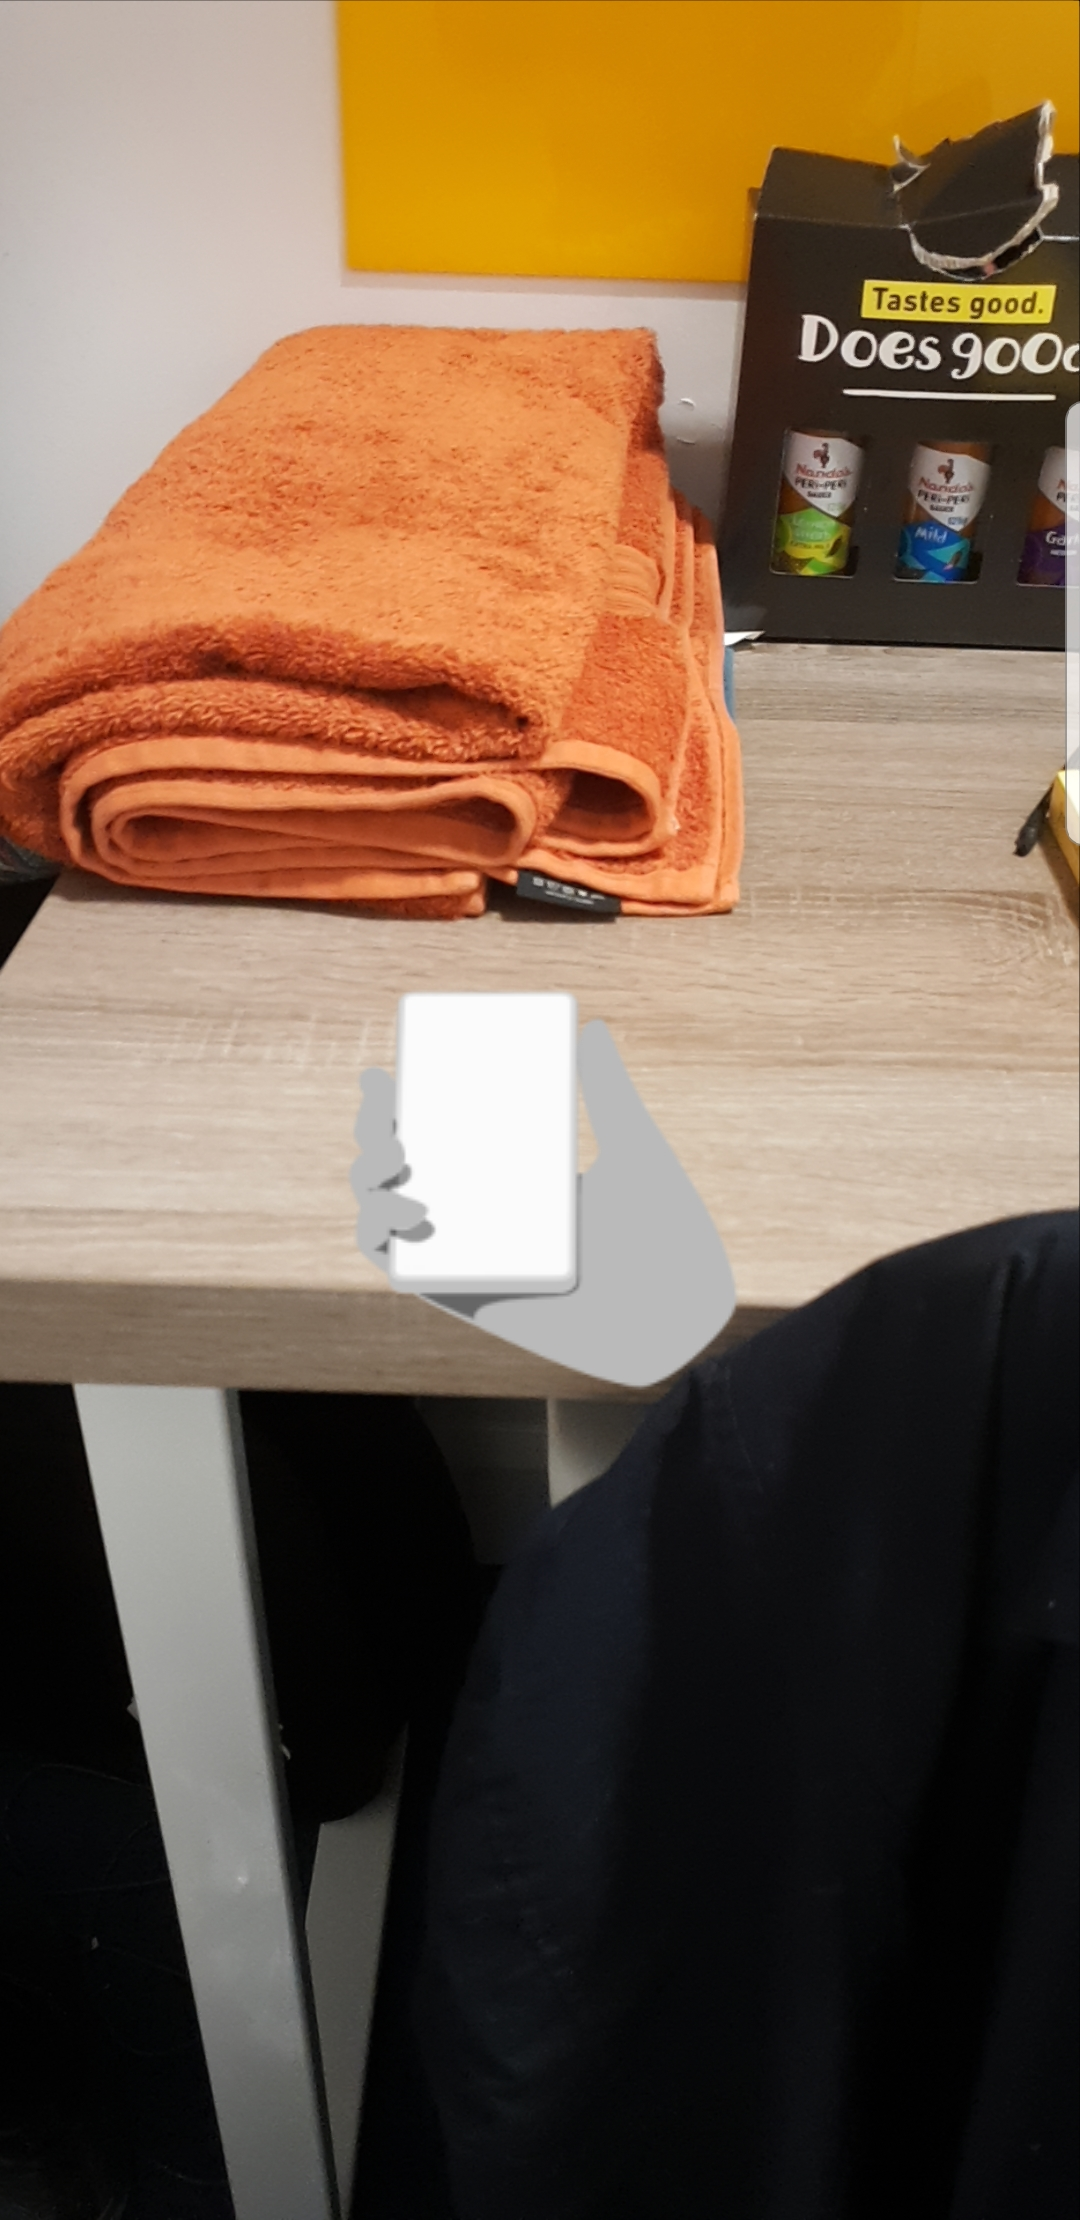
\includegraphics[width=60mm, height=100mm]{prototypes/ar/android/1.jpg} &   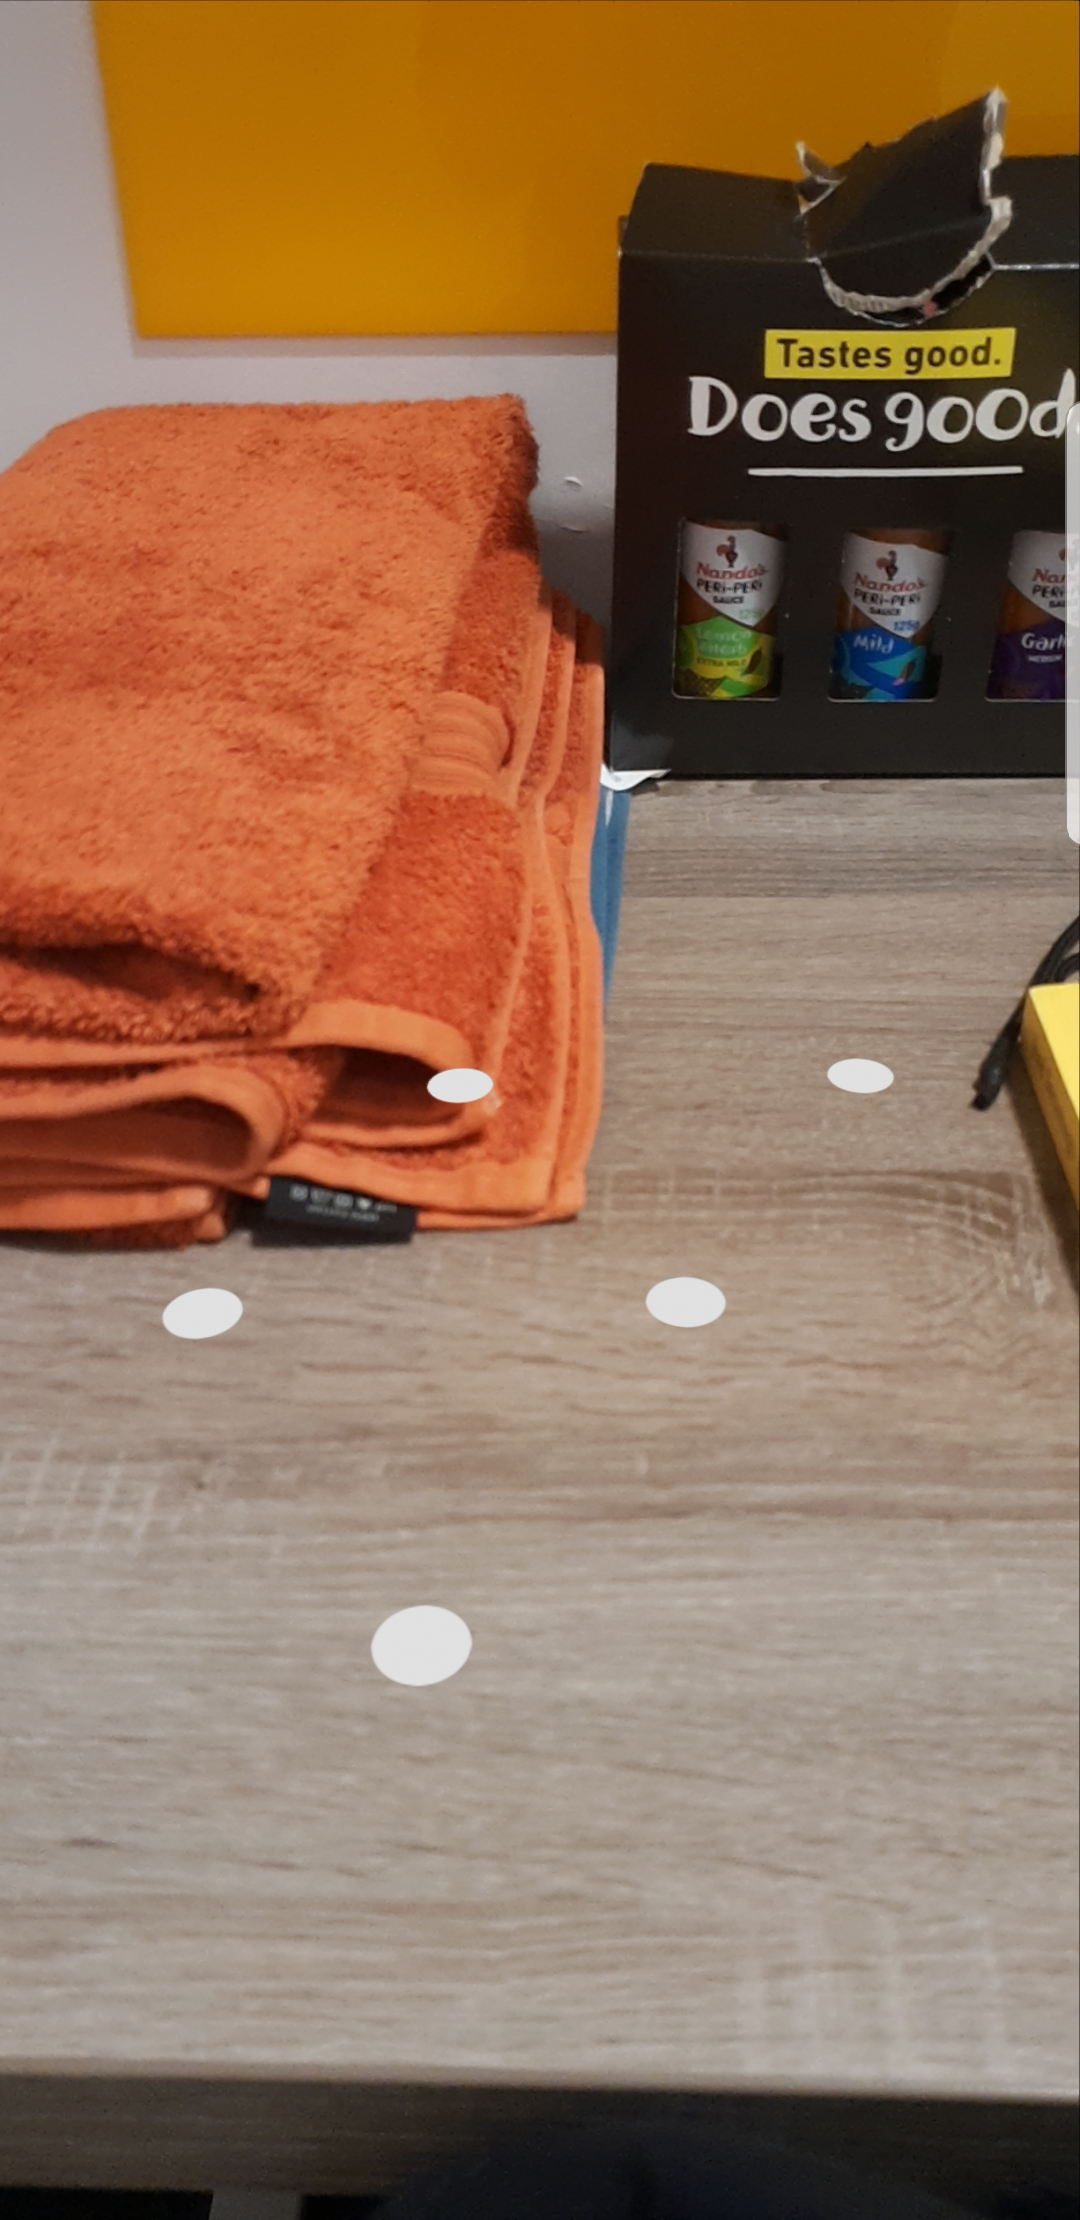
\includegraphics[width=60mm, height=100mm]{prototypes/ar/android/2.jpg} \\
% (a) Initial view & (b) Detection of surface \\[6pt]
% \multicolumn{2}{c}{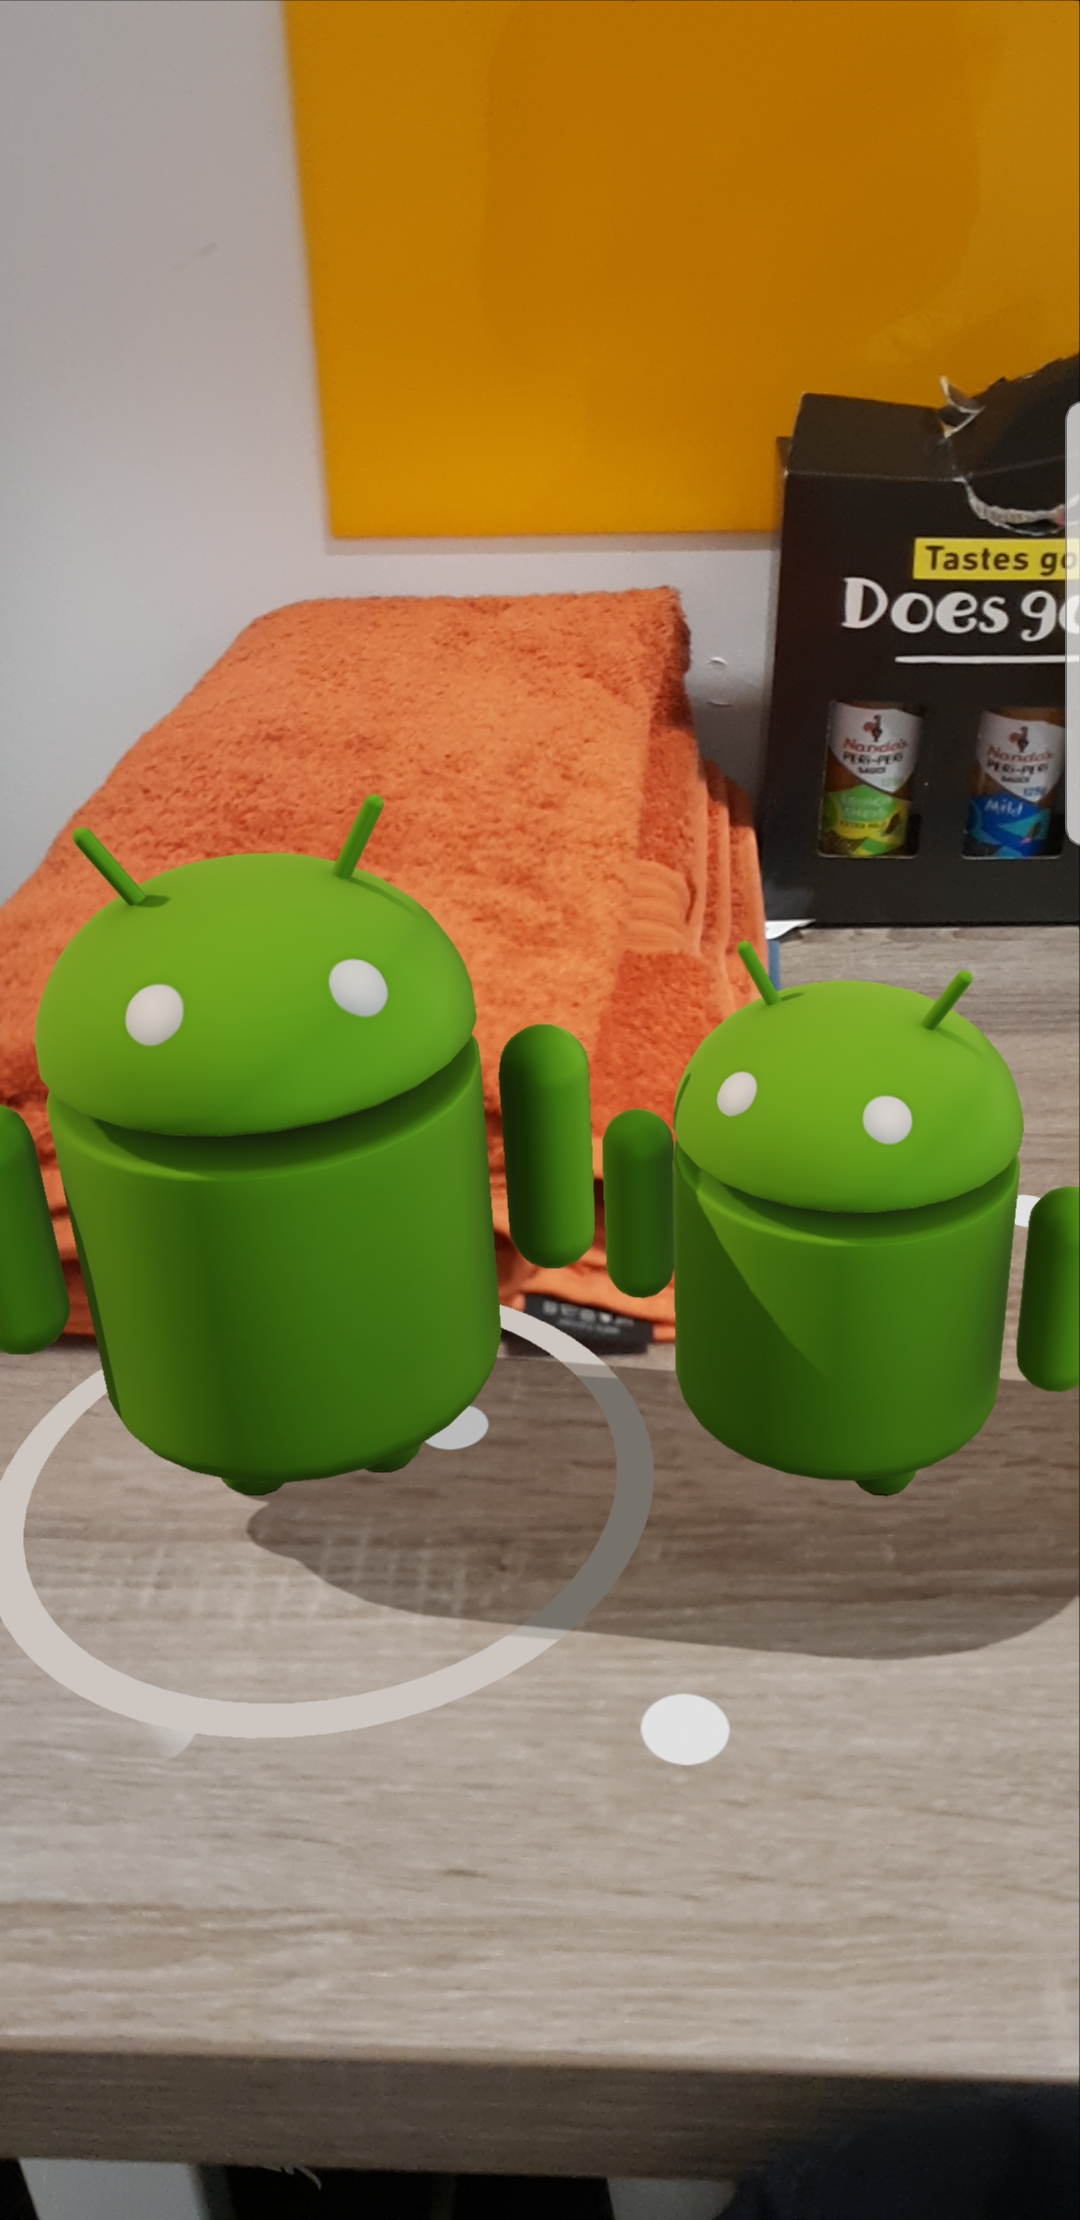
\includegraphics[width=60mm, height=100mm]{prototypes/ar/android/3.jpg} }\\
% \multicolumn{2}{c}{(c) Objects superimposed on surface}
% \end{tabular}
% \caption{ARCore prototyping on Android device}
% \label{fig:ARCore}
% \end{figure}

\section{Hardware - Arduino and Raspberry Pis}
Nick Week 1

As part of our exploration it was recommended, based off lengthy research and from our interlocution \remove{and other communication from}{with} \change{our professional partner}{the project's domain expert}, in-trusting to the chief organ of the project \note{doesn't make sense}, where location data would be derived from, to a physical beacon. 

This role of this beacon, no matter \change{is}{the} configuration was to broadcast a signal. \remove{There were many perfectly plausible methods for this put to us.} Three main \remove{recipes}{current technologies} exist: optical infra-red, Bluetooth and, \remove{lastly,} WiFi. Speaking to industry specialists, the former – which underpins their navigation technology and would yield pin-point accuracy – important if you are dealing with small indoor spaces, but this is expensive; Bluetooth, while less accurate, \remove{it} is far cheaper to manufacture and develop; the latter-most, WiFi offers the least in accuracy and not too expensive. From this probing, Bluetooth became the team’s \remove{favourite} solution.

Turning in to more a physical project which \change{wasn't}{was not} anticipated \remove{the extent of this}, \annote{we}{no third person} needed to design a beacon. Looking at relatable past projects, the favourable direction was using a Arduino (UNO R3 Mega 2560) or the Raspberry Pi 3 Model B+. Both solutions gave us a clear, small, and light-weight canvas on which to design our beacon. However, with a smaller physical footprint – also in keeping with the project’s eco-friendly policy, the Arduino was cheaper. This was a priority for us as we want our technology to have a wide-spread appeal. 

Taking forward the Arduino platform, \annote{we}{no first person} kitted it out with a Bluetooth HC-05 RF transceiver. This setup was able to broadcast a simple Bluetooth signal where we were able to decipher a signal strength from which we could determine a distance. Despite this, it became apparent that we would need to have further invested in more beacons to give a more accurate and reliable result via triangulation. This \change{wasn't}{was not} a suitable solution as one underpinning goal of this project is to make our technology assessable and available to a wide range of applications – an increase in cost would hinder this.
\note{can we add some photos of the arduino we used?}